% main4.tex -- H-main.  Section 4: walking the front; the end theorem (proved in Appendix A).
%======================================================================
\section{Walking the front: the end theorem}\label{sec:chase}
%======================================================================

This section is about the second act alone. Suppose Harry stands on a smooth front that is nearly straight at every
small scale. He walks along it in legs: from his current point he aims at the point an arclength $\varepsilon$ further
on and runs straight at it until he meets it. Everything he passes is within $\varepsilon$ of him, so it is seen. The
end theorem says that, if the front is flat enough to begin with, it \emph{stays} flat for the whole walk, every leg
makes progress at least $\varepsilon/\kappa$ along the front, and the walk ends after a time comparable to the length
of the front. We first define the walk precisely; throughout, $x$ is a working front on $[0,U]$ started at $t_\td$
with $|\partial_ux^0|\equiv1$, and a \emph{pair} $(a,b)$, $a<b$, has \emph{label length} $\lambda:=b-a$.

\begin{definition}[Greedy chase]\label{def:chase}
Let $P$ be $1$-Lipschitz on $[0,t_\td]$ with $x^0(0)=P(t_\td)$, and fix a \emph{cut} $b_c\in(0,U]$. Set
$t_0:=t_\td$ and $a_0:=0$. Given a leg start $t_j$ with $P(t_j)=x_{a_j}(t_j)$, let
\[
a_{j+1}:=\max\bigl\{u\in[a_j,b_c]:\ l_{t_j}(a_j,u)\le\varepsilon\bigr\}.
\]
If $a_{j+1}=b_c$, the chase stops at $T_\stopp:=t_j$ (leg $j+1$ is \emph{final} and is not walked; $P$ stays constant
after $T_\stopp$). Otherwise $P$ runs at unit speed along the ray from $P(t_j)$ through $x_{a_{j+1}}(t_j)$ until it
meets $x_{a_{j+1}}$, at time $t_{j+1}$; this requires the \emph{proviso} $c(a_j,a_{j+1};t_j)>0$. Leg $j+1$ is the time
interval $[t_j,t_{j+1}]$ and its direction is $\hat u_{j+1}$. For $t\in(t_j,t_{j+1}]$ (and for $t=t_0$, with $j=0$),
the label $a_{j(t)}:=a_j$ is the \emph{base} at time $t$.
\end{definition}

During a leg the target point flees straight away from Harry along his line of motion, so he gains on it at rate at
least $1-v$ and a leg lasts at most $\varepsilon/(1-v)$; every true label between $a_j$ and $a_{j+1}$ is within
$\varepsilon$ of Harry at the leg start, hence seen. These and other basic facts about the chase are collected in
Lemma~\ref{lem:chase} (Appendix~A).

\textbf{The setting.} The end theorem is used twice (once on a short initial arc, once on the whole front), and it must
tolerate the excused pairs near the tail end mentioned in Section~\ref{sec:idea}. This is what the following setting
encodes. The admissible pairs are those of label length between $\varepsilon/2$ and $R$ that are still ahead of Harry.
On a first reading one may take $\We=0$: then there are no tail pairs, $\mathcal F_*=\mathcal F$ below, and (TW) is
void; the excused tail is needed only in Section~\ref{sec:assembly}.

\textbf{Setting (H).}\phantomsection\label{set:H} Fix the locked parameters (with either $\gamma=\frac23$ or
$\gamma=\gamma_D=\frac34$), $M:=mR^{-\gamma}$, $U\le U_0:=8$, $\varepsilon\le R/K_\varepsilon$, the chase of
Definition~\ref{def:chase} on the working front $x$ on $[0,U]$ \emph{with cut $b_c=U$}, and an \emph{excuse
length} $\We\ge0$ (either $\We=0$ or $U\ge2\We+R+\varepsilon$), together with a number $\delta_t\ge0$ (in the application
$\delta_t=O_R(v)$; only $\delta_t\le\frac1{16}$ is used). A pair $(a,b)\subset[0,U]$ is a \emph{body pair} if
$U-b\ge\We$, a \emph{tail pair} if $U-b<\We$, and \emph{good} if $a\ge\We$ or $U-b\ge\We$ (every pair with $\lambda\le R$
is good). The \emph{family} $\mathcal F(t)$ on leg $j+1$ consists of the pairs with $\varepsilon/2\le\lambda\le R$ and
($a=a_j$ or $a\ge a_{j+1}$); pairs starting strictly inside the current leg are left out because their first point was
within $\varepsilon$ of Harry at the leg start and is therefore already seen. The \emph{gap} of a family pair is
$g:=a-a_{j(t)}\ge0$, and the pair is \emph{far} if $g\ge K_f\lambda$ and \emph{near} otherwise. Let $j_W$ be the first $j$ with $a_j\ge\We$, and $t_W:=t_{j_W}$. The \emph{admissible
family} $\mathcal F_*(t)$ consists of the body pairs of $\mathcal F(t)$ for $t<t_W$, and of all of $\mathcal F(t)$ for
$t\ge t_W$. Assume:
\begin{itemize}
\setlength{\itemsep}{2pt}\setlength{\parskip}{0pt}
\item[(S1)] $c(a,b;t_\td)\ge c_A\min(\lambda,K_RR)$ for all good pairs with $\lambda\ge\varepsilon/2$;
\item[(S2)] $N(a,b;t_\td)\le s_0M\lambda^{1/2+\gamma}\min\bigl(1,\,K_f\lambda/\min(a,K_RR)\bigr)^\nu$ for all body
pairs with $\varepsilon/2\le\lambda\le R$;
\item[(TW)] (if $\We>0$ and $t_W$ is reached) every tail pair with $\varepsilon/2\le\lambda\le R$ satisfies, with
$g_W:=a-a_{j_W}$,
\[
g_W\ge K_f\lambda,\qquad l_{t_W}(a,b)\le(1+\delta_t)\lambda,\qquad
N(a,b;t_W)\le s_0M\lambda^{1/2+\gamma}\min\Bigl(1,\,\frac{K_f\lambda}{\min(g_W,K_RR)}\Bigr)^\nu .
\]
\end{itemize}
The weight $\min(\cdot)^\nu$ in (S2) and (TW) asks a pair that starts far ahead of Harry to be slightly flatter; this
pays for the logarithmic amplification $\int v\,dt/g$ that it suffers while Harry approaches (see ``Far pairs'' below).

\begin{theorem}[End theorem]\label{thm:end}
In Setting~\textup{(H)}, provided $v_0=v_0(m,R)>0$ is sufficiently small, the proviso holds at every non-final leg
start, and:
\begin{enumerate}[(a)]
\setlength{\itemsep}{1pt}\setlength{\parskip}{0pt}
\item \textup{(Invariants)} For all $t\in[t_\td,T_\stopp]$ and all $(a,b)\in\mathcal F_*(t)$,
\begin{equation}\label{eq:invariants}
\text{\textup{(J1)}}\quad l_t(a,b)\le\kappa\lambda,\qquad\text{\textup{(J2)}}\quad N(a,b;t)\le M\lambda^{1/2+\gamma};
\end{equation}
if $\We>0$, then $t_W$ is reached. Moreover $c(a,b;t)\ge c_A\min(\lambda,K_RR)$ for all good pairs with
$\lambda\ge\varepsilon/2$.
\item \textup{(Termination)} Every non-final leg advances the base by $a_{j+1}-a_j\in[\varepsilon/\kappa,\varepsilon]$;
the chase stops by $T_\stopp\le t_\td+\kappa U/(1-v)$; and every true label of $[0,U]$ is seen by $T_\stopp$.
\item \textup{(Tilts)} For $J\subset I$ in $\mathcal F_*(t)$: $|e_J-e_I|\le C_TM\lambda_I^\gamma$, with the absolute
constant $C_T:=\sqrt5\,(1-2m^2)^{-1/2}/(1-2^{-\gamma})$ \textup($C_T<6.11$ for $\gamma=\frac23$, $C_T<5.58$ for
$\gamma=\frac34$\textup).
\item \textup{(Distance from the base)} On leg $j+1$, for $s\ge a_j$ with $U-s\ge\We$ or $a_j\ge\We$:
$\rho_s(t)\ge c_A\min(s-a_j,K_RR)-\delta_1\varepsilon$ and $\max(\rho_s(t),\varepsilon)\ge\min(s-a_j,K_RR)/c_6$, where
$c_6:=(1+\delta_1)/c_A=\frac92$.
\item \textup{(Causality)} If $\tilde P=P$ on $[0,t_j]$, then \textup{(a)}, \textup{(c)}, \textup{(d)} hold for
$\tilde P$ on $[t_\td,t_j]$.
\end{enumerate}
\end{theorem}

The proof is in Appendix~A. Here is why it works.

\textbf{A first-failure argument.} The invariants (J1)--(J2) hold at $t_\td$ with room to spare, by (S1)--(S2). Both
sides change continuously in time, so if they ever fail there is a first moment when one of them becomes an equality.
It therefore suffices to show that, as long as (J1)--(J2) hold, they actually hold in the \emph{strictly stronger} forms
$l<\kappa\lambda$ and $N^2\le\bar\theta M^2\lambda^{1+2\gamma}$ for a fixed $\bar\theta<1$ (Lemma~\ref{lem:cont}). The
invariants are exactly what keeps the chase healthy: (J1) makes every leg advance the base by at least $\varepsilon/\kappa$,
so the walk ends in time about $\kappa U$; and (J2), via the split-tilt lemma, keeps all chords pointing in nearly the
same direction, so Harry is never far off the line of the pairs ahead of him. Three estimates give the strict forms.

\emph{Far pairs} (Proposition~\ref{prop:far}). A pair whose distance ahead of Harry is at least $K_f=10$ times its own
length sees Harry from far away. The regularisation plays no role there, and the far inequality and the Duhamel
inequality (Lemmas~\ref{lem:Eprime}(iv) and \ref{lem:duhamel}) apply. The amplification factor $\exp\int\mathcal A$
involves $\int v\,dt/g$, which grows only logarithmically as the gap $g$ shrinks; the factor $\min(\cdot)^\nu$ in (S2) is
designed to absorb exactly this logarithm. The forcing $\mathcal B$ is small because Harry is nearly on the line of the
pair: his sideways
offset $|p_a|$ is controlled by the bendiness of a longer pair reaching back to him. The result is
$N\le f_FM\lambda^{1/2+\gamma}$ with $f_F=\frac12$.

\emph{Near pairs} (Proposition~\ref{prop:near}). A pair close to Harry may feel the singular part of the field, but
only briefly: Harry moves past it at speed about $1$, so it is near for a time of order $\lambda$, and the integral of
the excess growth over that time is bounded by a constant times $vM^2\lambda^{1+2\gamma}$, with a constant that does
not depend on $\varepsilon$. The point is that the time spent at gap $g$ can be traded for an integral over $g$,
because consecutive legs move the base by at least $\varepsilon/\kappa$: sums over legs of (leg duration)$\times h(g)$ are
bounded by $\kappa d_L\int h(g)\,dg$, and $\varepsilon$ cancels. So the bendiness inherited from the far phase,
at most $f_F^2/2$ in units of $M^2\lambda^{1+2\gamma}$, grows by only $O(v)$.

\emph{Length} (Proposition~\ref{prop:length}). The same bookkeeping shows that the length of an admissible pair grows
by a factor $1+O_R(v)$ at most, so it stays below $\kappa\lambda$.

Figure~\ref{fig:timeline} shows this life cycle in a simulation: a pair is far for most of the walk, and its bendiness
barely moves; then Harry approaches and passes it, and the bendiness takes a small kick.

\begin{figure}[!htbp]
\centering
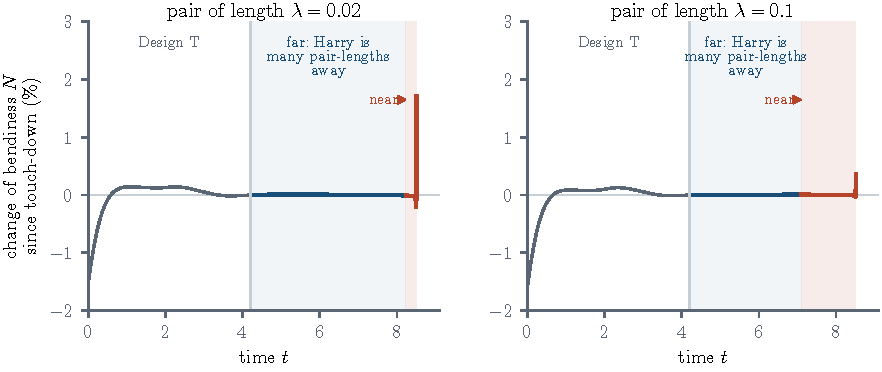
\includegraphics[width=0.95\linewidth]{figs/fig_timeline.pdf}
\caption{The life of two pairs of points on the front during a simulated walk of the kind shown in
Figure~\ref{fig:designT}, here with $v=0.1$ and $\varepsilon=0.01$ (Figure~\ref{fig:designT} itself uses
$\varepsilon=0.02$): relative change of their bendiness $N$ since touch-down. The pairs are labelled by direction; the
indicated $\lambda$ is their length in direction, and their arclength at touch-down is about $1.1\lambda$ (the far/near
test uses arclength). While the pair is far ahead of Harry (blue), $N$ hardly changes. When Harry comes within ten
pair-lengths (red), $N$ moves by at most two percent before Harry passes the pair and sees it.}
\label{fig:timeline}
\end{figure}

\textbf{Where $\varepsilon$ enters.} Only in three ways, each harmless: every pair considered has $\lambda\ge\varepsilon/2$;
$\varepsilon\le R/K_\varepsilon$; and each leg lasts at most $d_L\varepsilon$ while moving the base by at least
$\varepsilon/\kappa$, which converts time integrals into gap integrals. This is why $v_0$ and the time bound in
Theorem~\ref{thm:end} do not depend on $\varepsilon$.
